% ISBI 2027 4-page paper, draft of 1 November 2026. Template: ISBI_template-master (spconf.sty, IEEEbib.bst).
\documentclass{article}
\usepackage{spconf,amsmath,amssymb,graphicx}
\usepackage{booktabs}
\usepackage[hidelinks]{hyperref}
\usepackage{enumitem}
\setlist{nosep, leftmargin=12pt}
\newtheorem{prop}{Proposition}
\newcommand{\todo}[1]{\textbf{[#1]}}

\title{The identity ladder: calibrating image similarity against matched strangers}
\name{Ekaterina Kondrateva$^{1,2}$, Florian Kofler$^{1,3,4,5}$}
\address{$^{1}$Hertie Institute for AI in Brain Health, University of T\"ubingen, Germany\\
$^{2}$Department of Radiation Oncology (Maastro), GROW, Maastricht University, The Netherlands\\
$^{3}$Department of Quantitative Biomedicine, University of Zurich, Switzerland\\
$^{4}$Helmholtz AI, Helmholtz Munich, Germany\quad $^{5}$TUM School of Medicine and Health, Technical University of Munich, Germany}

\begin{document}
\maketitle

\begin{abstract}
Similarity metrics such as SSIM, PSNR and RMSE are read as evidence that a synthesized region, a harmonized scan or a reconstructed face keeps an individual's anatomy, but their values carry no identity scale. We define an identity ladder of reference pairs (same sitting, another day, another device, years apart, the contralateral side, monozygotic and dizygotic co-twins, unrelated people) and score a pair by its placement among unrelated pairs matched on acquisition nuisance. Under an additive variance-component model the expected score of a rung has a closed form, $P(F_{D,D}>\rho)$, in the rung's variance ratio $\rho$, from which test--retest reliability and twin heritability follow. The model predicts failure modes of current metrics: squared error ranks an identity-free population-average fill above a co-twin's tissue whenever the genetic share of variance is below one half, SSIM rewards flat fills in low-contrast regions, and in the BraTS inpainting ranking PSNR repeats RMSE. Synthetic ladders with known components and three open iris and fundus datasets confirm these predictions.
\end{abstract}
\begin{keywords}
image similarity, metric validation, inpainting, twins, test--retest reliability
\end{keywords}

\section{Introduction}
\label{sec:intro}
Inpainting~\cite{kofler2023brats}, harmonization, image translation~\cite{dohmen2025} and re-identification~\cite{nebbia2025} are judged with pairwise similarity between an output and a reference image. A value such as SSIM $=0.9$ is then read as ``close to the real individual'', yet nothing in the metric says how close a re-scan of the same person, a twin or a stranger would be in the same setting. Raw values shift with intensity normalization, mask size and region contrast, so the same number can mean a re-scan in one dataset and a stranger in another; metric selection frameworks catalogue such pitfalls but do not supply an identity scale~\cite{maierhein2024}.

Other fields calibrate similarity against unrelated pairs: TM-score against random protein structures~\cite{zhang2004}, speaker verification against impostor cohorts~\cite{auckenthaler2000}, diagnostic markers by placement values among controls, adjusted for covariates~\cite{pepe2005,janes2009}, and test--retest pipelines by discriminability~\cite{bridgeford2021}. Brain imaging has reported ordered similarities from retest to twins to strangers for specific features~\cite{yeh2016}. We combine these elements into one scale and analyse existing metrics on it. Our contributions are (i) the identity ladder with a nuisance-matched calibrated score and a nuisance-only negative control; (ii) closed forms under a variance-component model that connect the rungs to reliability, heritability and bilateral asymmetry and predict three failure modes of standard metrics; (iii) checks on synthetic ladders, including 2D tissue scored with the official BraTS inpainting code~\cite{inpainting2026}, and on three open datasets.

\section{Method}
\label{sec:method}
\subsection{Identity ladder and calibrated score}
A rung is a relation between two acquisitions, defined by what they share: the same sitting (L0), another day (L0$'$), another device (L1), years apart (L2), the other body side (mirror), a monozygotic (MZ) or dizygotic (DZ) co-twin (L3), or nothing (L4, strangers). For any distance $d$ (a metric oriented so that smaller is more similar), the calibrated score of a pair is
\begin{equation}
c(d)=P(d_{\mathrm{ref}}>d)+\tfrac12 P(d_{\mathrm{ref}}=d),
\label{eq:c}
\end{equation}
where $d_{\mathrm{ref}}$ is drawn from stranger pairs in the same nuisance stratum (device pair, time gap, body side). This is a placement value with a covariate-matched reference~\cite{pepe2005,janes2009}: strangers score $1/2$, and the mean of $c$ over a rung is its AUC against matched strangers. Because $c$ depends on $d$ only through ranks, MSE, RMSE and PSNR give the same $c$. A nuisance-only feature (for images, the global mean and SD of intensity) is scored on the same ladder as a negative control~\cite{lipsitch2010}.

\subsection{Variance-component model}
An acquisition of side $s$ of person $p$ in sitting $k$ at time $t_k$ is $x=g_p+e_p+b_{ps}+a_p t_k+\eta_{pk}+n+\varepsilon$, with independent zero-mean Gaussian components in $D$ dimensions: genotype $g$ (shared fully by MZ and with correlation $1/2$ by DZ co-twins), individual development $e$, side-specific development $b$, ageing slope $a$, sitting nuisance $\eta$, device nuisance $n$ (present on device B) and noise $\varepsilon$, with variances $\sigma_\cdot^2$ per dimension. The difference of two acquisitions is Gaussian with per-dimension variance $v_r$: $v_{\mathrm{L0}}=2\sigma_\varepsilon^2$, $v_{\mathrm{L0'}}=2(\sigma_\varepsilon^2+\sigma_\eta^2)$, $v_{\mathrm{L1}}=v_{\mathrm{L0'}}+\sigma_n^2$, $v_{\mathrm{L2}}=v_{\mathrm{L0'}}+\sigma_a^2\Delta t^2$, $v_{\mathrm{mir}}=2(\sigma_b^2+\sigma_\varepsilon^2)$ within a sitting, $v_{\mathrm{MZ}}=2(\sigma_e^2+\sigma_b^2)+v_{\mathrm{L0'}}$, $v_{\mathrm{DZ}}=v_{\mathrm{MZ}}+\sigma_g^2$ and $v_{\mathrm{L4}}=2V$ with $V=\sigma_g^2+\sigma_e^2+\sigma_b^2+\sigma_\eta^2+\sigma_\varepsilon^2$; strangers matched to L1 or L2 carry the same extra terms.

\begin{prop}[closed form]
With $\rho_r=v_r/v_{\mathrm{ref}(r)}$, $\mathbb{E}\,c_r=P(F_{D,D}>\rho_r)=I_{1/(1+\rho_r)}(D/2,D/2)$, where $I$ is the regularized incomplete beta function.
\end{prop}
\noindent\emph{Proof.} $d_r^2/v_r$ and $d_{\mathrm{ref}}^2/v_{\mathrm{ref}}$ are independent $\chi^2_D$ variables, so $d_{\mathrm{ref}}^2/d_r^2\cdot\rho_r\sim F_{D,D}$. $\square$

\begin{prop}[classical quantities]
$1-\rho_{\mathrm{L0'}}$ is the test--retest ICC of the features~\cite{shrout1979}; $2(\rho_{\mathrm{DZ}}-\rho_{\mathrm{MZ}})=\sigma_g^2/V$, the twin estimator of heritability in distance form~\cite{polderman2015}; and $\rho_{\mathrm{mir}}\le\rho_{\mathrm{MZ}}$, so under additivity the contralateral side never ranks below an MZ co-twin.
\end{prop}

\begin{prop}[dimension]
For fixed $\rho<1$, $\mathbb{E}\,c$ rises with $D$, so $c$ is not comparable across feature spaces of different effective dimension. The moment ratio $\hat\rho_r=\overline{d_r^2}/\overline{d_{\mathrm{ref}}^2}$ is free of $D$, and $D_{\mathrm{eff}}=2\,\overline{d^2}^{\,2}/\mathrm{Var}(d^2)$ over strangers estimates $D$, as degrees of freedom do for iris codes~\cite{daugman2004}.
\end{prop}

\begin{prop}[pooled reference, negative control]
Scoring L1 pairs against same-device strangers lowers $v_{\mathrm{ref}}$ by $\sigma_n^2$ and biases $c_{\mathrm{L1}}$ down, exaggerating the cost of a device change. A nuisance-only feature $\eta+\varepsilon$ gives $c=1/2$ on every rung that crosses sittings but $P(F_{D,D}>\sigma_\varepsilon^2/(\sigma_\varepsilon^2+\sigma_\eta^2))>1/2$ within one sitting, which is the share of same-sitting similarity that is not identity.
\end{prop}

\subsection{Failure modes of standard metrics}
\begin{prop}[squared error rewards the average]
For a masked region of $x$ filled with $f$, $\mathbb{E}\|x-f\|^2/D$ equals $V$ for the leave-one-out population mean, $2V$ for a stranger's tissue, $2V(1-h^2)$ for an MZ co-twin's tissue with $h^2=\sigma_g^2/V$, and $2(\sigma_b^2+\sigma_\varepsilon^2)$ for the contralateral side in the same sitting. An identity-free fill therefore beats MZ tissue whenever $h^2<1/2$ and reaches $c=P(F_{D,D}>1/2)>1/2$ without any individual anatomy, so the floor for a fill is the population-mean score, not $1/2$. Rescaling a template to the target's SD adds variance and removes the effect.
\end{prop}

\begin{prop}[SSIM stabilizer]
For a fill that is constant within an SSIM window, $\mathrm{SSIM}=l\cdot C_2/(\sigma_x^2+C_2)$~\cite{wang2004} with $C_2=(0.03L)^2$, data range $L$ and luminance term $l$. Where the local SD of the reference is well below $0.03L$, a mean-matched flat fill scores close to 1 regardless of identity.
\end{prop}

\begin{prop}[BraTS ranking]
In the challenge code~\cite{inpainting2026} the PSNR data range comes from the reference inside the mask, so within a case PSNR is a decreasing function of the error and repeats the RMSE order, except that plain PSNR first clamps the fill to that range. The case-wise rank-sum with equal weights over SSIM, PSNR and RMSE~\cite{kofler2023brats} therefore weights squared error two thirds.
\end{prop}

\section{Experiments}
\label{sec:experiments}
\textbf{Synthetic vectors.} 300 twin families (half MZ), two sides, four sittings (baseline, another day, device B, one time unit later) and two repeats; $D\in\{8,32\}$; component SDs $(g,e,b,a,\eta,n,\varepsilon)=(1,0.6,0.5,0.5,0.3,0.6,0.4)$ (genetic share $0.54$) and a second set with $g=0.6$, $e=1$ (genetic share $0.19$). Proposition~2 is checked on 2000 families with a family bootstrap.
\textbf{Synthetic tissue.} $64\times64$ images: a smooth template plus Gaussian random fields for $g$, $e$, $b$ (scales of 2--3 pixels), a global offset per sitting and white noise; identity contrast $\times1$ or $\times0.2$; 60 families; masks of $32^2$ and $12^2$ pixels. Fills are the rung partners, the leave-one-out population mean with and without SD matching, and 16 stranger fills per case, all scored with the official BraTS metric code (inpainting 0.0.12; torchmetrics 1.1.2 and 1.9.0 gave identical results on our checks); $c$ is computed per case against the stranger fills.
\textbf{Open data.} UPOL~\cite{dobes2004} (64 people) and UTIRIS NIR~\cite{hosseini2010} (78 people) iris images with repeats from one sitting and both eyes; GRAPE~\cite{huang2023grape} fundus photographs (144 patients, three cameras, visits months apart) with released RETFound features~\cite{nebbia2025}. Features: the nuisance-only control, $16\times16$ pixels, a classical iris code with Hamming distance~\cite{daugman2004}, and RETFound. References are stratified by device pair and eye relation; intervals are 95\% person-cluster bootstrap intervals, conditional on the reference.

\section{Results}
\label{sec:results}
\begin{figure*}[t]
\centering
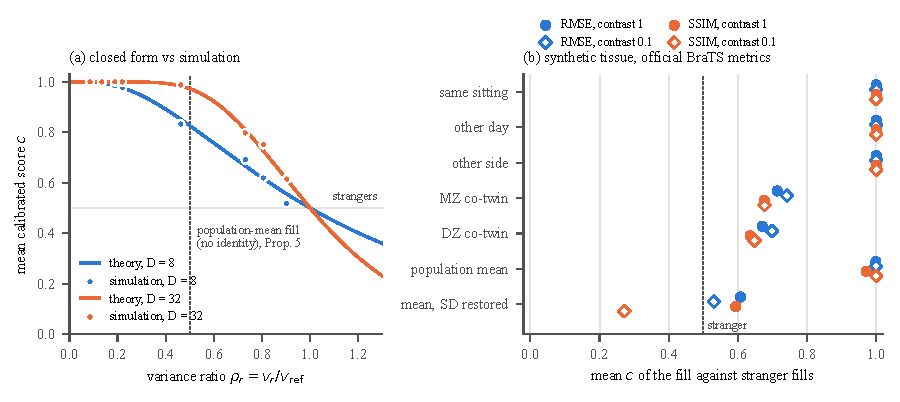
\includegraphics[width=\textwidth]{fig_ladder.pdf}
\caption{(a) Simulated mean $c$ of every rung (dots) against the closed form of Proposition~1 (lines), two parameter sets, $D=8$ and $32$. (b) Synthetic 2D tissue, genetic share $0.19$, $32^2$ mask: mean $c$ of each fill against 16 stranger fills under RMSE and SSIM (official BraTS code), identity contrast $\times1$ (filled) and $\times0.2$ (open). The identity-free population mean outranks both co-twins under RMSE and every rung under SSIM at low contrast.}
\label{fig:ladder}
\end{figure*}

\textbf{Closed forms.} Across all rungs, parameter sets and both dimensions, simulated mean $c$ differed from Proposition~1 by at most $0.037$ (Fig.~\ref{fig:ladder}a). The effective dimension estimated from strangers was $7.5$--$7.9$ for $D=8$ and $32.2$--$32.7$ for $D=32$. On 2000 families, $2(\hat\rho_{\mathrm{DZ}}-\hat\rho_{\mathrm{MZ}})$ recovered the genetic share: $0.525$ [0.477, 0.579] and $0.531$ [0.503, 0.560] for a true $0.538$ ($D=8$, $32$), and $0.187$ [0.115, 0.254] and $0.220$ [0.187, 0.256] for a true $0.194$. The nuisance-only control scored $0.723$ within a sitting (theory $0.729$) and $0.500$ across sittings.

\textbf{Failure modes.} On synthetic tissue with genetic share $0.19$, the population-mean fill reached $c=1.00$ under RMSE, against $0.72$ for MZ and $0.64$ for DZ co-twin tissue; with genetic share $0.54$, MZ tissue and the mean fill tied ($0.97$ and $0.99$), as Proposition~5 predicts at $h^2\approx1/2$. With SD matching the template fell to $c\le0.02$. At identity contrast $\times0.2$, SSIM gave the flat mean fill $c=0.99$ while all real rungs, including the same person on another day, scored $0.52$--$0.65$ (Fig.~\ref{fig:ladder}b). Raw anchors moved with the mask: the median stranger SSIM was $0.56$ with the $32^2$ mask and $0.89$ with the $12^2$ mask, and stranger PSNR $10.6$ against $8.5$\,dB, while $c$ stays anchored at $1/2$ by construction. On synthetic checks of the official code, MSE, PSNR$_\epsilon$, PSNR$_{01}$ and PSNR$_{01,\epsilon}$ ranked fills exactly as RMSE did (Kendall $\tau=1$), plain PSNR with $\tau=0.89$ because of its clamping, and SSIM was computed per 2D slice of a volume.

\begin{table}[t]
\centering
\caption{Open data: mean $c$ against matched strangers [95\% CI].}
\label{tab:real}
\footnotesize
\begin{tabular}{@{}llll@{}}
\toprule
Data & Feature & Same eye, same sitting & Fellow eye \\
\midrule
UPOL & nuisance only & 0.919 [0.900, 0.936] & 0.884 [0.861, 0.904] \\
UPOL & pixels & 0.923 [0.899, 0.944] & 0.819 [0.782, 0.853] \\
UTIRIS & nuisance only & 0.793 [0.769, 0.818] & 0.764 [0.741, 0.784] \\
UTIRIS & iris code & 0.913 [0.889, 0.938] & 0.677 [0.635, 0.718] \\
\midrule
\multicolumn{4}{@{}l}{GRAPE, RETFound: drop in $c$ for a camera change at another visit} \\
\multicolumn{4}{@{}l}{\quad pooled reference $0.260$ [0.183, 0.329]; matched reference $0.096$ [0.048, 0.146]} \\
\bottomrule
\end{tabular}
\end{table}

\textbf{Open data.} The nuisance-only control, two numbers per image, reached $c=0.92$ (UPOL) and $0.79$ (UTIRIS) for same-sitting repeats and $0.88$ and $0.76$ for the fellow eye (Table~\ref{tab:real}), as Proposition~4 predicts for shared sittings: on these sets most of the pixel-level similarity is exposure. The iris code rose above the control for the same eye ($0.913$) and fell below it for the fellow eye ($0.677$), consistent with $\rho_{\mathrm{mir}}$ close to 1 for iris texture~\cite{daugman2004}. Near-identical acquisitions can likewise explain claimed re-identification from foundation-model features~\cite{engelmann2026}. On GRAPE a pooled stranger reference made a camera change cost $0.26$ in $c$, against $0.10$ with a camera-matched reference.

\section{Discussion and conclusion}
\label{sec:discussion}
A similarity value becomes interpretable once it is placed among matched strangers and next to the rungs of the same person, a contralateral side and twins; the repeat rungs bound what a metric can resolve, as rater variability does for segmentation metrics~\cite{kofler2023pgt}. The model explains why the same metric looks good or bad in different settings: squared error rewards the population mean, SSIM's stabilizer rewards flat fills where contrast is low, and pooled references and shared sittings inflate or deflate scores. We recommend reporting $c$ with a matched reference, the score of the population-mean fill as the floor, the nuisance-only control, and $\hat\rho$ for comparisons across feature spaces. Limitations: the model is Gaussian and additive (dominance and non-Gaussian tails change the twin rungs), the open data have no twins and no repeats across days, and per-case references of 16 fills are coarse. Next steps are twin cohorts with zygosity and an MRI donor-swap test of BraTS inpainting methods, in which healthy masks are filled with tissue from a re-scan, a co-twin and a stranger. Code and synthetic data will be released.

\section{Compliance with ethical standards}
\label{sec:ethics}
This study used synthetic data and three publicly available, de-identified datasets (UPOL, UTIRIS, GRAPE) released by their original investigators; no new data were collected. \todo{To confirm: ethics approval or waiver for the secondary use of these data, and the wording required by the Hertie Institute.}

\section{Acknowledgments}
\label{sec:acknowledgments}
\todo{Funding.} The authors declare no conflicts of interest \todo{to confirm}. Claude (Anthropic) was used to write and test the analysis code, to search and check literature and dataset sources, and to draft the text of all sections; the authors checked the derivations, the numbers against the released results and the final text.

\bibliographystyle{IEEEbib}
\bibliography{refs}
\end{document}
